\chapter{Method}
\label{sec:method}

We propose a method for constructing a similarity model from an unlabeled dataset that contains a small proportion of approximately labeled instances. This method is applied on our use case of 3D CAD models, but it is actually generalizable to other domains. 

Unlabeled triplets are generated from the entire dataset \autoref{sec:triplet-generation}. These triplets are then labeled using a dedicated application \autoref{sec:labeling-application}. Finally, the labeled triplets are used to train a model based on triplet loss \autoref{sec:triplet-loss-training}.


\section{Labeling application}
\label{sec:labeling-application}

Before delving into the details of the pipeline, it is essential to introduce the user interface that has been developed in order to build the labeled triplets database.

There are actually two main use cases for the application: labeling triplets (\autoref{fig:labeling_use_case}) and comparing two iterations of a model (\autoref{fig:validation_use_case}).

\begin{itemize}
  \item \textbf{Labeling triplets:} Users are presented with a triplet of 3D models, with the reference model (anchor) in the center. Their task is to swipe left or right to indicate whether the left or right model is more similar to the anchor model. A skip option is also available for ambiguous cases.
  
  Users can also change to a canonical view of the models to facilitate the comparison. This changes the perspective of a camera to a view aligned with the model's principal axes. This may or may not be useful depending on the model's geometry, as shown in \autoref{fig:default_vs_canonical}.

\begin{figure}[]
  \centering
  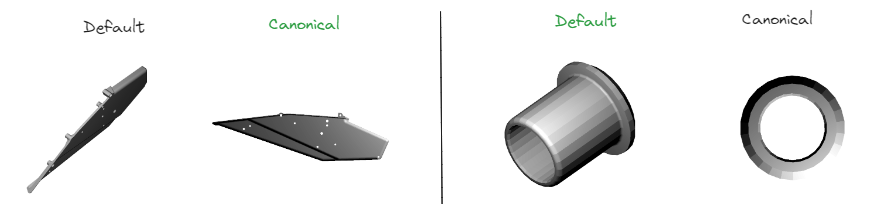
\includegraphics[width=\columnwidth]{images/default_vs_canonical.png}
  \caption{Two pieces where the appropriate view is different.}
  \label{fig:default_vs_canonical}
\end{figure}

  Additional metadata is also provided to the users, such as the piece length. This information can help users make more informed decisions when the geometry does not suffice.
  %TODO: change model to piece everywhere
  \item \textbf{Validation:} A similar interface is used, but now the propositions on the left and right are two nearest neighbors propositions of two different models. Users judge which model gives the best nearest neighbor proposition. This gives an easy way to compare two iterations of a model. This is especially useful to bulletproof the model's performance, ensuring robustness not only in quantitative metrics but also in qualitative assessments.
  
\end{itemize}

\begin{figure}[]
  \centering
  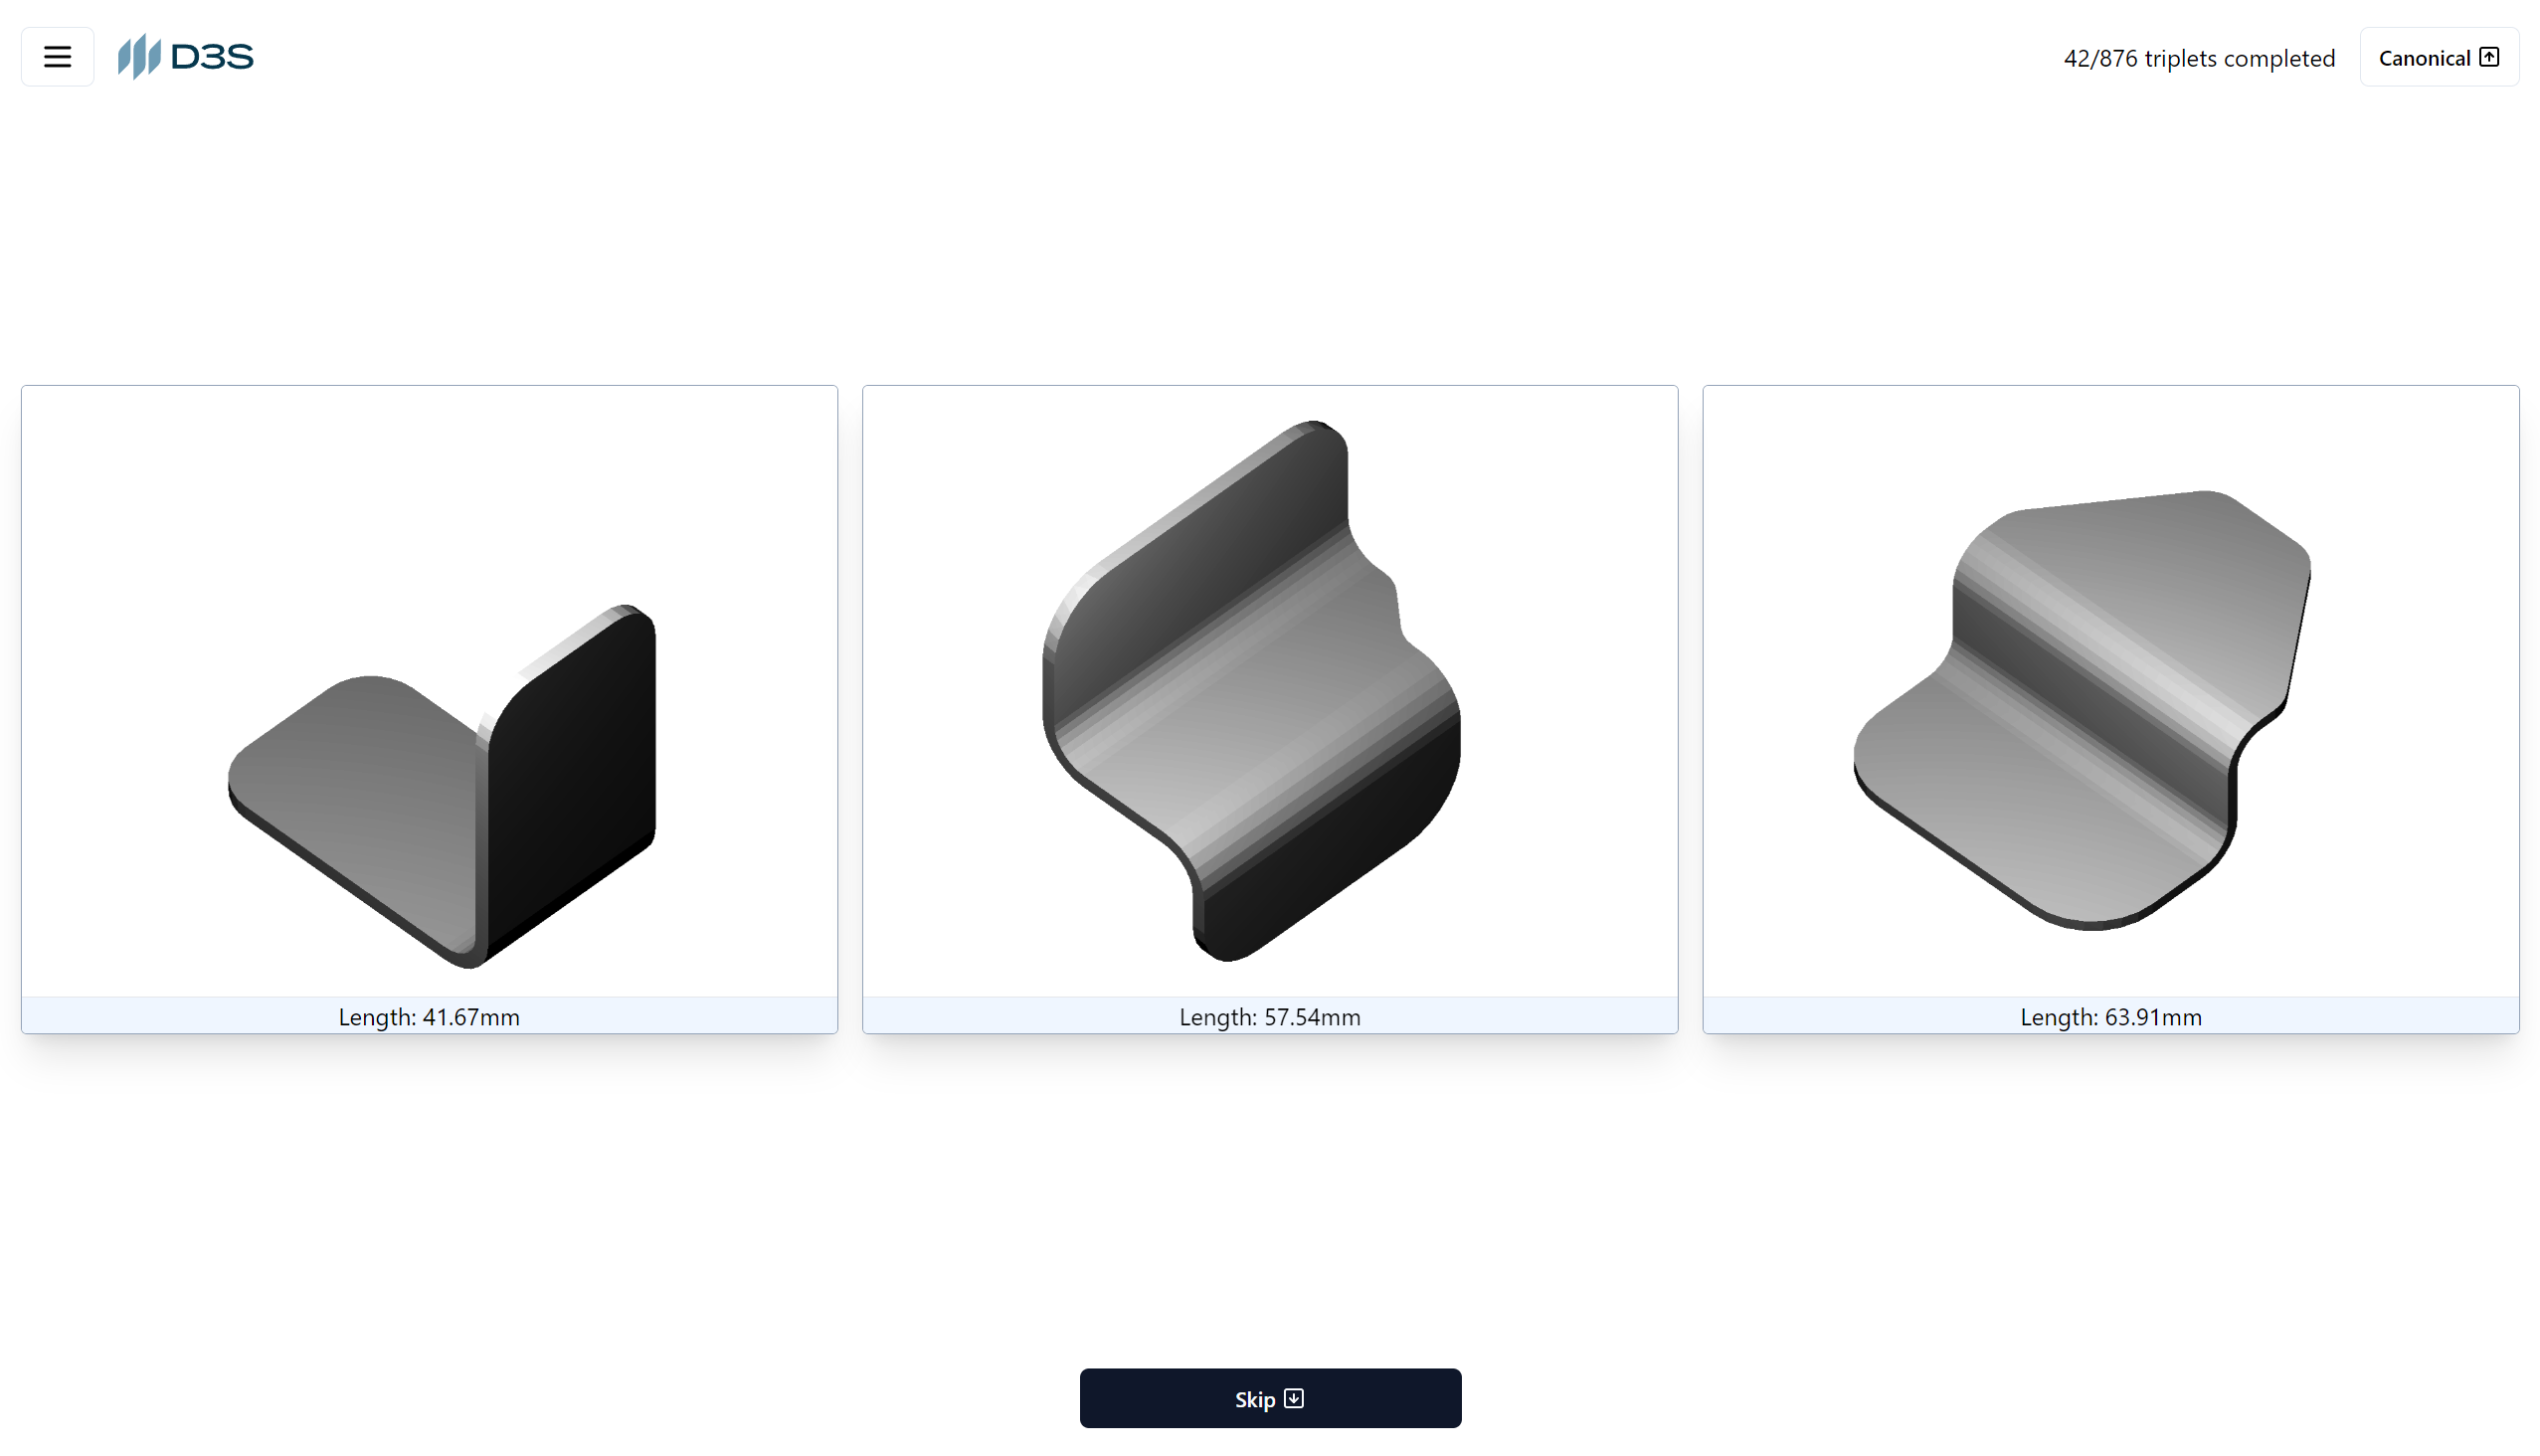
\includegraphics[width=0.8\columnwidth]{images/tinder3d_labeling.png}
  \caption{User interface for the labeling use case. Here, the piece on the right is more similar to the anchor piece in the center (curved edges).}
  \label{fig:labeling_use_case}
\end{figure}

\begin{figure}[]
  \centering
  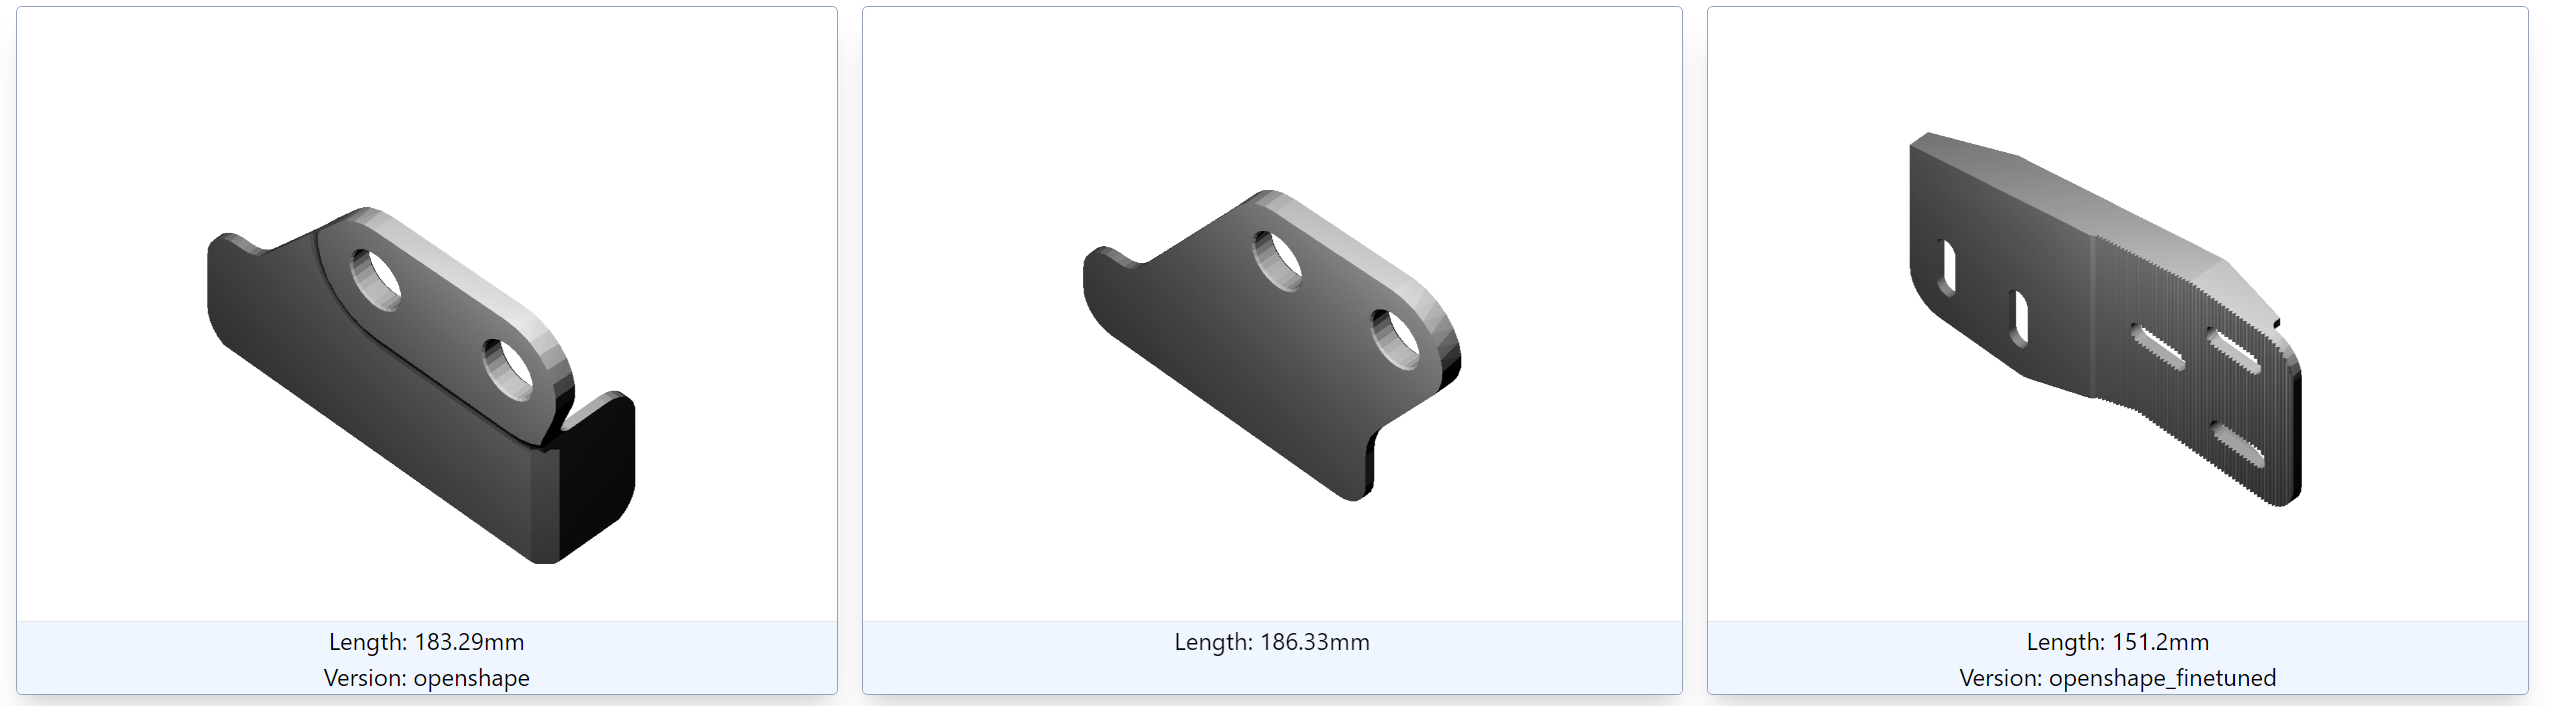
\includegraphics[width=0.8\columnwidth]{images/tinder3d_validation.png}
  \caption{User interface for the validation use case. Here, the proposition of the model on the left is more similar to the anchor piece in the center (two holes at the top).}
  \label{fig:validation_use_case}
\end{figure}

This application is designed to be intuitive and user-friendly, allowing users to quickly and efficiently label triplets.

Additional gamification elements were considered at one point, but they were deemed unnecessary as we were already achieving strong results with a small number of triplets.

\section{Triplet loss training}
\label{sec:triplet-loss-training}

The goal is to learn a representation of data such that similar instances are close together in the representation space, while dissimilar instances are far apart. We are going to use a triplet loss approach to train our encoder model. Once we will have our embeddings, the \textbf{cosine similarity} will be used to define a distance among the data points.

$$d(x, y) = 1 - \frac{x \cdot y}{\|x\| \|y\|}$$

The loss will be defined over triplets of embeddings:
\begin{itemize}
  \item An anchor.
  \item A positive, of the same class as the anchor.
  \item A negative, of a different class than the anchor.
\end{itemize}

\vspace{0.2cm}

Given a batch size $N$, a distance function $d$, a margin $margin$ and $a$, $p$ and $n$ tensors representing anchor, positive and negative examples, respectively.

$\ell(a, p, n)=L=\left\{l_1, \ldots, l_N\right\}^{\top}, \quad l_i=\max \left\{d\left(a_i, p_i\right)-d\left(a_i, n_i\right)+\text { margin }, 0\right\}$

Input tensors $a$, $p$ and $n$ are of shape $(N, D)$, where $D$ is the embedding dimension. The loss $l_i$ is computed for each triplet in the batch, and the final loss is the mean of all individual losses.

Intuitively, you aim to group the data into separate clusters, ensuring that each class forms its own cluster. However, the precise distance between clusters isn't a concern, as long as they remain clearly distinct. Without limiting the loss, the model could improve by pushing an easy negative example very far away, while neglecting more challenging negative examples. By capping the reward beyond a certain distance, the model is encouraged to focus on the harder examples to continue improving.

Based on the definition of the loss, there are three categories of triplets:
\begin{itemize}
  \item \textbf{Easy triplets:} Triplets which have a loss of $0$, because $d(a, p) + margin < d(a, n)$.
  \item \textbf{Hard triplets:} Triplets where the negative is closer to the anchor than the positive, i.e. $d(a, n) < d(a, p)$.
  \item \textbf{Semi-hard triplets:} Triplets where the negative is not closer to the anchor than the positive, but which still have positive loss: $d(a, p) < d(a, n) < d(a, p) + margin$.
\end{itemize}

\begin{figure}[]
  \centering
  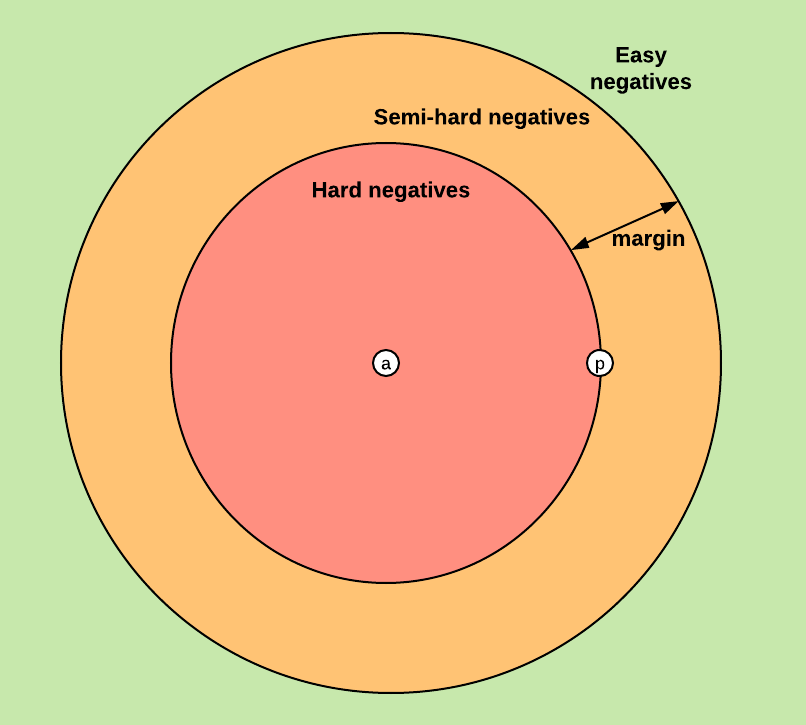
\includegraphics[width=0.5\columnwidth]{images/negative_types.png}
  \caption{The three types of negatives, given an anchor and a positive.}
  \label{fig:negative_types}
\end{figure}

The balance of these triplet types is crucial for the model's performance, as we will see in TODO.

Before delving deeper into working on triplet loss, we had to first ensure that training a triplet loss model with 'fake triplets' generated from our labeled dataset yielded similar results to a classification model trained on the same dataset. To do so, a GNN based on the EdgeConv architecure \cite{wangDynamicGraphCNN2019} was used. 

The performance of the classification model was evaluated against the triplet loss model using a nearest neighbor approach. This method assessed how often a piece's label matched that of its closest neighbor in the learned representation space. Both models achieved a 95\% accuracy rate, suggesting that the triplet loss model successfully learned to create meaningful representations of the data. It is important to emphasize that at this point only triplets generated from the labels were used, and no human labeling was done. Triplets are generated following the same approach as in \autoref{sec:triplet-generation-heuristics}, but ensuring that the anchor and the positive are indeed of the same class. 

With just 1000 triplets, the model achieved a nearest neighbor accuracy similar to the classification model. However, optimal performance was observed when using approximately 10000 triplets, which resulted in a 95\% accuracy rate.

\section{Triplets generation}
\label{sec:triplet-generation}

There is still the question of how to generate the triplets that are going to be labeled by the user of the app. Let's draw the properties of the triplets we want to generate, ordered by ease of implementation:
\begin{enumerate}
  \item The triplets should be diverse enough to cover the entire dataset.
  \item Almost every triplet should be 'labelable'. A triplet is 'labelable' if users do not have to skip it. This is a mainly a user experience concern. 
  \item A great proportion of triplets should be 'hard triplets' for the model that generated them, ie triplets where the negative is hard. This will force the next iteration of the model to learn from its misconceptions.
\end{enumerate}


A simple yet effective way has been proposed to generate triplets. For the initial generation, a model trained on the small labeled dataset we had was used to compute embeddings for the entire dataset. This model was used to generate triplets based on heuristics which are detailed in \autoref{sec:triplet-generation-heuristics}. Subsequently, the model was retrained on the labeled triplets, and the process was repeated iteratively.

With such a method, property 1 is straightforward to achieve, as a random selection of triplets will cover the entire dataset. Property 2 and 3 are in conflict, as a triplet that is easy to label is likely to be easy for the model as well. Considering the limits, selecting candidates that are equidistant from the anchor is intriguing, but tends to result in many 'skipped' triplets. Conversely, choosing candidates where the first is closer than the second will lead to fewer skipped triplets, but also a lower proportion of semi-hard and hard triplets.

It's why a proper balance has to be found, as explained in \autoref{sec:triplet-generation-heuristics}.

%%% Local Variables: 
%%% mode: latex
%%% TeX-master: "isae-report-template"
%%% End: 